\subsection{\'{E}tude des performances d'une batterie de voiture électrique}
%tiré de Mines-Pont 2022.

\setcounter{equation}{0}
\setcounter{Q}{0}

Les batteries utilisées couramment dans les véhicules électriques, mais également dans d'autres applications comme les téléphones portables, sont de type lithium-ion. Elles présentent l'avantage d'avoir une très grande énergie massique, comprise entre 90 et \SI{180}{\watt\hour\per\kilo\gram}. De plus, ces batteries, même partiellement déchargées, délivrent toujours la même puissance, ce qui permet une utilisation dans les mêmes conditions, quel que soit le niveau de charge. Le principe général d'une batterie lithium-ion est basé sur l'échange réversible des ions lithium entre une électrode positive en oxyde métallique (\ce{MO2}) et une électrode négative en graphite qui va stocker les ions lithium pendant la charge :

~

\begin{minipage}[c]{0.65\textwidth}
\centering
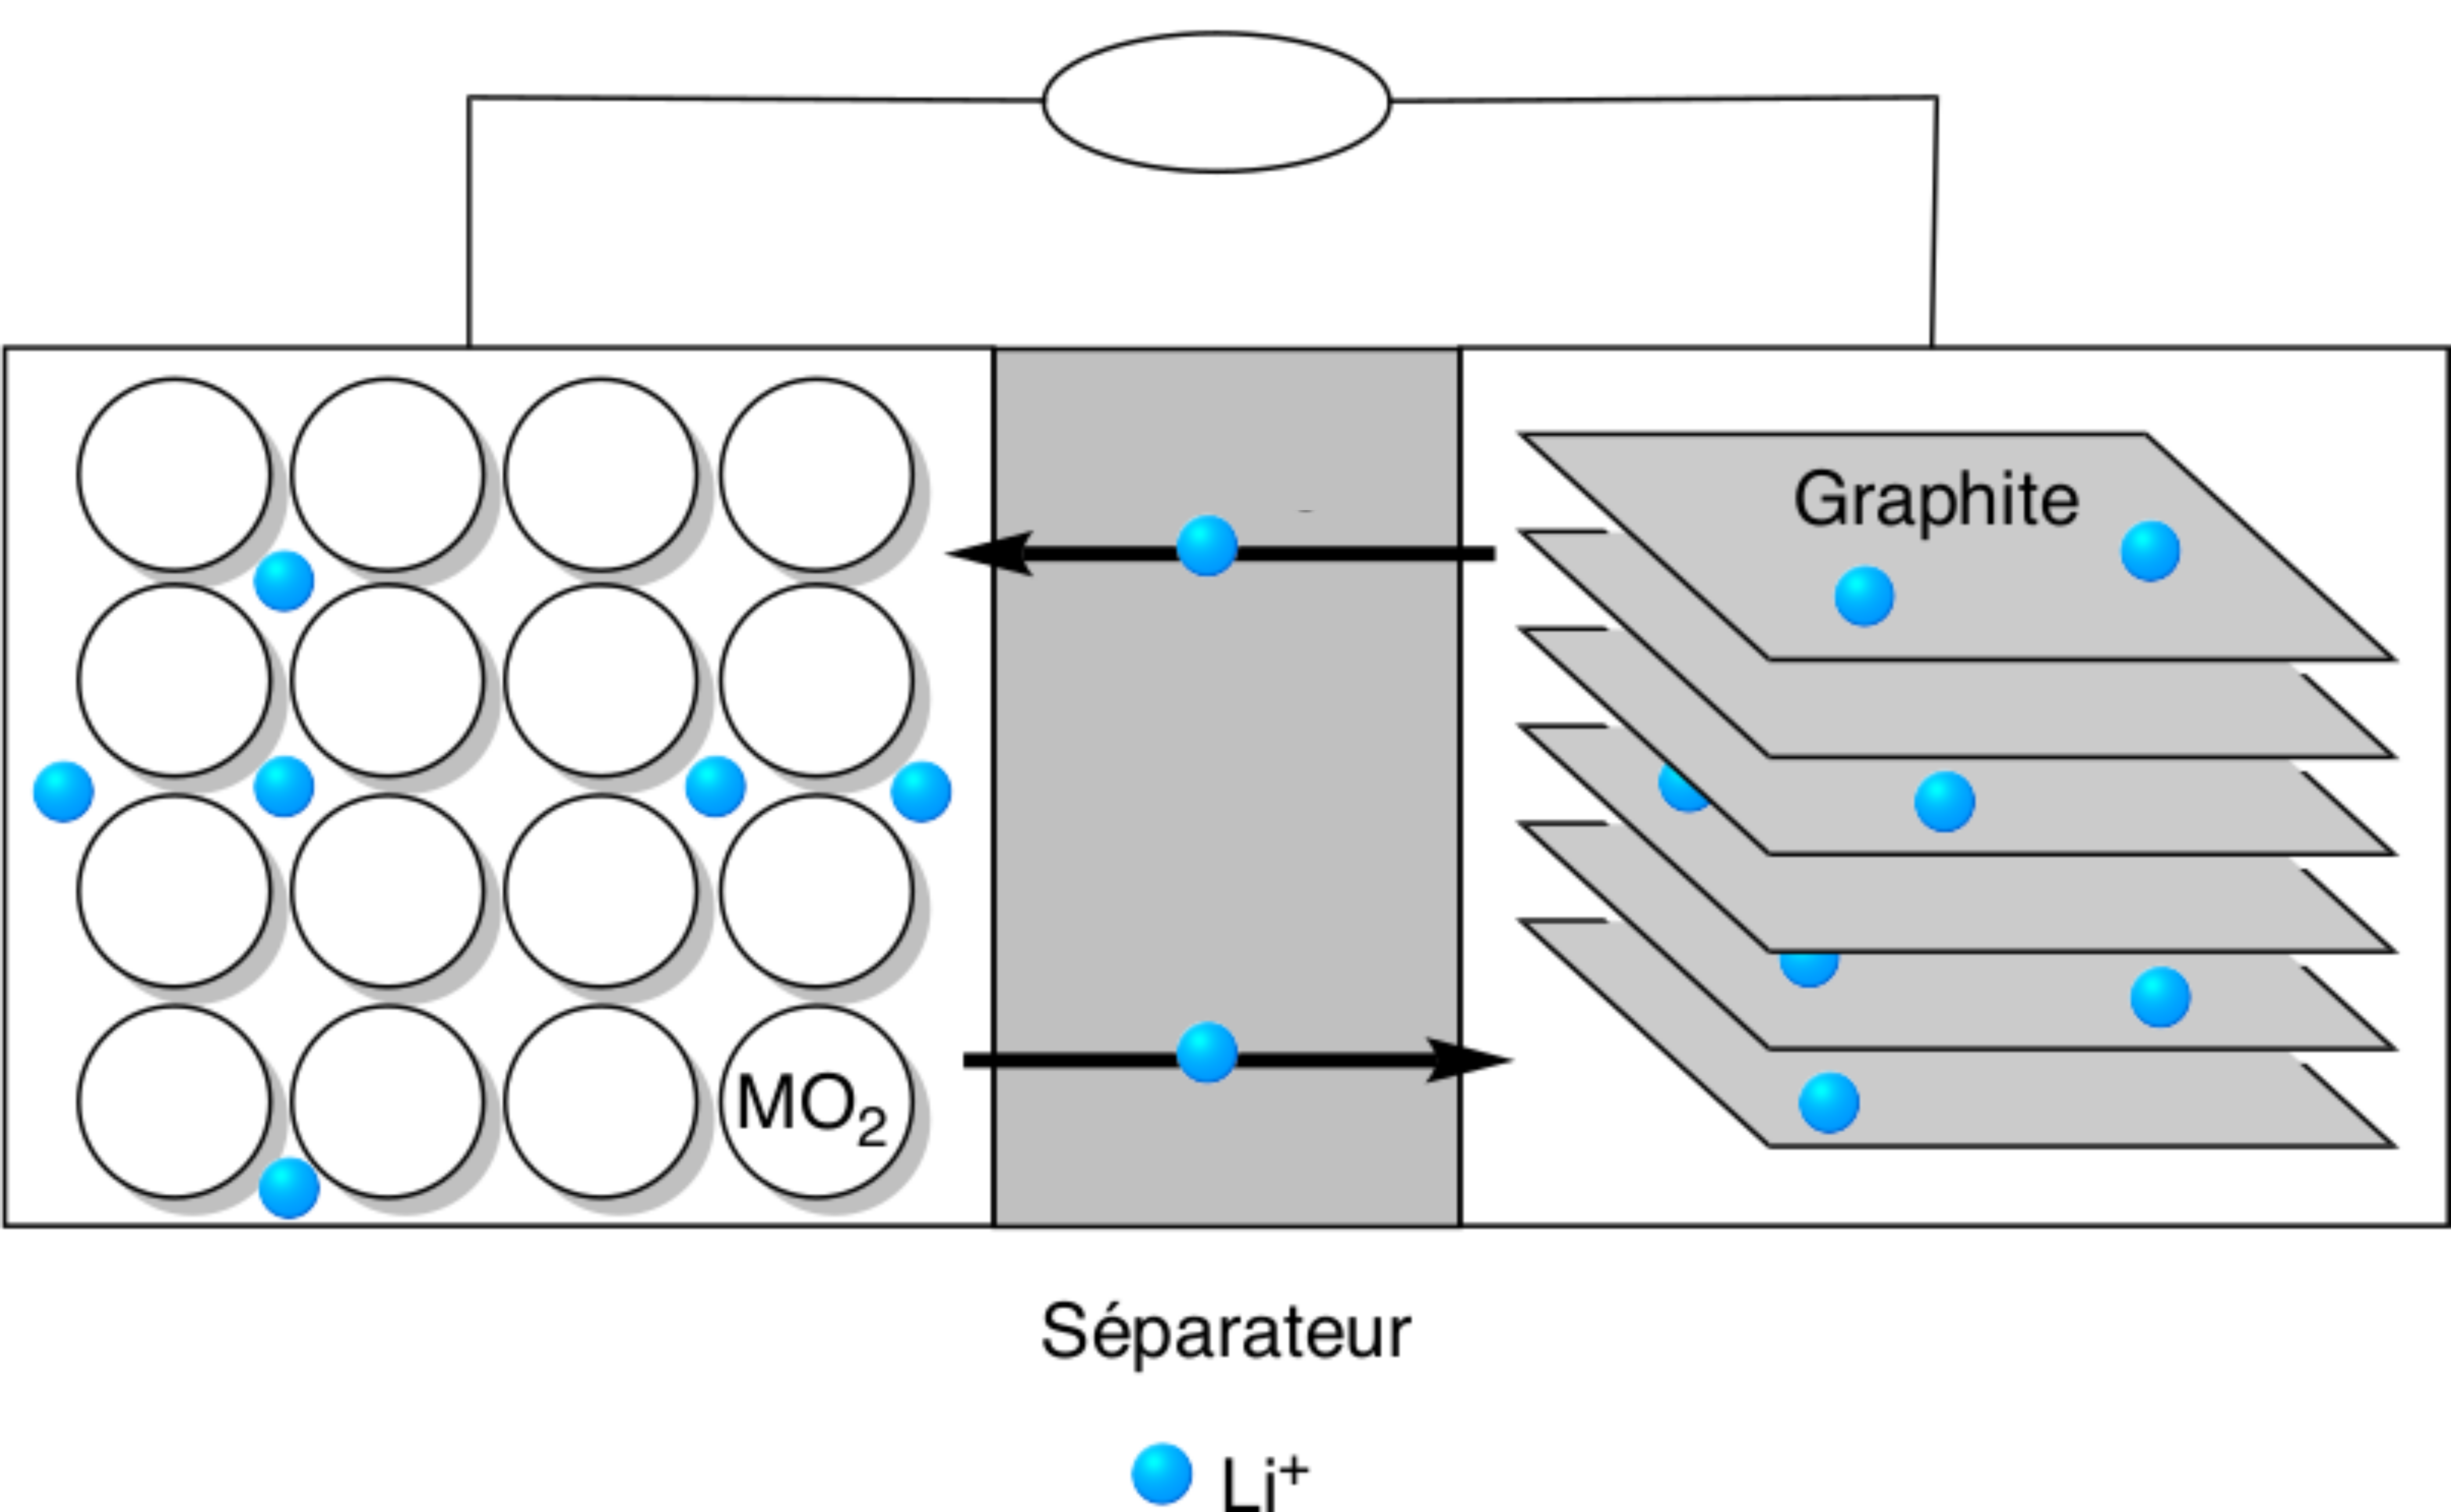
\includegraphics[width=6cm]{Ex22/7-BatteryLithium.png}
\end{minipage}\hfill   
\begin{minipage}[c]{0.35\textwidth}     
\captionof{figure}{Technologie au lithium-ion. Le solvant utilisé est une espèce organique.}
\label{fig:22-01}
\end{minipage}

\Q En vous appuyant sur la représentation du graphite Fig. \ref{fig:22-02}, expliquer pourquoi les ions Li peuvent s'insérer entre les feuillets de graphite. On sait que le rayon ionique du lithium est de \SI{60}{\pico\meter} et le covalent est de \SI{134}{\pico\meter}.

\begin{minipage}[c]{0.65\textwidth}
\centering
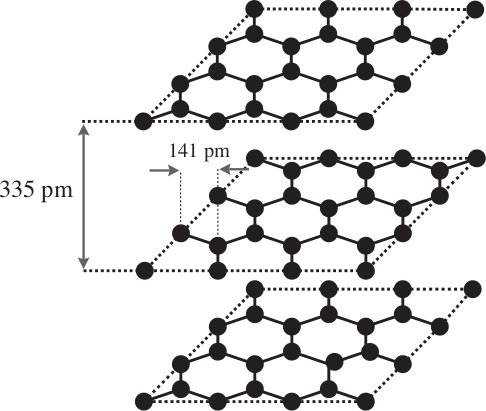
\includegraphics[height=4cm]{Ex22/11-graphene.png}
\end{minipage}\hfill   
\begin{minipage}[c]{0.35\textwidth}     
\centering
\captionof{figure}{Structure du graphite}
\label{fig:22-02}
\end{minipage}

\Q \`{A} l'état totalement chargé, la structure du composé est \ce{LiC6}. Écrire la demi-équation rédox à cette électrode lors de la charge et de la décharge et préciser le signe de l'électrode de graphite.
La seconde électrode peut être en dioxyde de cobalt (\ce{CoO2}) qui, après insertion des ions lithium,
forme l'oxyde lithié \ce{LiCoO2}. 
\solution{L'équation de la demi-pile en décharge est modélisée par : 
\begin{align*}
\ce{LiC6 = Li^+ + e^- + C_6}
\end{align*}
Il s'agit d'une oxydation, cette électrode est donc l'anode en décharge, donc le pôle $\ominus$ !}

\Q Montrer que l'élément cobalt change de degré d'oxydation au cours de la décharge. Commenter la valeur.
\solution{On peut évaluer les degrés d'oxydation du cobalt à l'état (SoC = \SI{100}{\percent}) chargé et déchargé (SoC = \SI{0}{\percent}). On résume les étapes dans un tableau : 
\begin{center}\begin{tabular}{ccccc}
SoC & pôle $\ominus$ & pôle $\oplus$ & Conservation charge & $no(\ce{Co})$ \\
\SI{100}{\percent} & \ce{LiC6} & \ce{CoO2} & $no(\ce{Co}) + 2 no (\ce{O}) = 0$ & IV \\ 
\SI{0}{\percent} & \ce{C6} & \ce{LiCoO2} & $no(\ce{Co}) + no(\ce{Li}) + 2no(\ce{O}) = 0$ & III
\end{tabular}\end{center}
car $\chi (\ce{Li}) < \chi (\ce{Co}) < \chi (\ce{O})$.\\
On trouve donc que $\Delta no(\ce{Co}) = -I$ pour une décharge totale. $\Delta no <0$ il s'agit bien d'une réduction.} 

\Q Donner la demi-équation électronique associée au couple considéré lors de la charge et de la décharge à cette électrode en précisant son rôle.
\solution{Différents processus au pôle $\oplus$ : 
\begin{center}
\begin{tabular}{ccc}
Processus & rôle & demi-équation rédox \\
décharge & cathode & \ce{Li^+ + e^- + CoO2 = LiCoO2} \\
charge & anode & \ce{LiCoO2 = Li^+ + e^- + CoO2}
\end{tabular}\end{center}
}
\Q Reproduire et orienter le schéma de la Fig. \ref{fig:22-01} dans le cas d'une charge puis d'une décharge. Vous indiquerez le nom et le signe des électrodes puis le flux d'électron, le courant électrique et la direction de migration des ions lithium.
\solution{On peut présenter deux schémas, un pour la charge, un pour la décharge en annotant tout ce qui est demandé.\\
\begin{minipage}{0.48\textwidth}
\begin{center}

\includegraphics[width=\textwidth]{Ex22/Corr01}
en charge
\end{center}
\end{minipage}\hfill\begin{minipage}{0.48\textwidth}
\begin{center}

\includegraphics[width=\textwidth]{Ex22/Corr02}
en décharge
\end{center}
\end{minipage}\\
On pensera en charge à positionner un générateur électrique (\emph{par ex.} une source de tension) et en décharge un récepteur électrique (\emph{par ex.} une résistance).}

\Q Déterminer l'expression de la capacité de la batterie (en \si{\ampere\hour\per\kilo\gram}) en fonction du nombre d'électrons échangés, de la constante de Faraday et de la masse molaire du matériau d'insertion (le graphite). Calculer sa valeur.
\solution{Encore une fois, on est emmené à dresser un tableau d'avancer : 
\begin{center}
\begin{tabular}{cccccccc}
\si{\mole} & \ce{LiC6} & \ce{ = } & \ce{Li^+} & \ce{ + } & \ce{e^-} & \ce{ + } & \ce{ C_6 }\\
$t=0$ & $n_0$ & & 0 & & 0 & & 0 \\
$t=\infty$ & $n_0-\xi_\infty$ & & $\xi_\infty$ & & $\xi_\infty$ & & $\xi_\infty$ \\
\end{tabular}\end{center}
Lorsque le matériau est totalement déchargé $SoC=0 ~ \si{\percent}$, il aura délivré $n_0 = \xi_\infty$ mol d'électrons et d'ion lithium. Par conséquent, pour une électrode de graphite de masse $m_{hote}$ et de masse molaire $M_{hote} = 6 M(\ce{C})$, on a alors : 
\begin{align*}
Q = F n_0 = F \xi_\infty = F \frac{m_{hote}}{6 M(\ce{C})}
\end{align*}
La capacité spécifique massique $C_m$ est la quantité de charge rammenée sur la masse du matériau hôte, soit : 
\begin{align*}
C_m  &= \frac{Q}{m_{hote}} = \frac{F}{6 M(\ce{C})} \quad [\si{\coulomb}]\\
&= \frac{F}{6 \cdot 3600 M(C)} \approx \frac{26.8}{6M(\ce{C})} \quad [\si{\ampere\hour\per\kilo\gram}]
\end{align*} 
avec $M(\ce{C})$ est exprimé en $\si{\kilo\gram\per\mole}$. \\
\textbf{AN :} $C_m = 372 \si{\ampere\hour\per\kilo\gram}$}

Pour le véhicule considéré, équipé d'une batterie lithium-ion dont les caractéristiques sont fournies dans le \textbf{Document}, la jauge d'autonomie de la batterie indique \SI{20}{\percent}. Son conducteur souhaite la recharger et pour cela, il utilise une borne de recharge qui fournit une puissance constante de \SI{7.40}{\kilo\watt} en délivrant un courant électrique d'intensité constante de \SI{32.0}{\ampere}.

\Q Calculer l'énergie massique maximale de la batterie considérée (\textbf{Document}). Commenter.
\solution{L'énergie massique maximale, notée $E_m$, est définie comme l'énergie utilisable, ramenée à la masse de la batterie : 
\begin{align*}
E_m = \frac{E}{m}
\end{align*}
où $E$ est l'énergie utilisable et $m$ la masse de la batterie.\\
\textbf{AN :} $E_m = 0.13 ~ \si{\kilo\watt\hour\per\kilo\gram} = 4.7 \cdot 10^5 ~ \si{\joule\per\kilo\gram}$ }

\Q Calculer l'énergie emmagasinée par la batterie lors de sa charge pour passer d'un SOC de \SI{20}{\percent} à \SI{80}{\percent} et définir le rendement énergétique de la charge, puis le calculer. Commenter cette valeur.

\solution{
On peut commencer par calculer le travail électrique reçu par la batterie (c.-à-d. délivré par la borne) : 
\begin{align*}
W_{recu}' &= \int_{t_{20}}^{t_{80}} P(t') dt' \\
&= P (t_{80} - t_{20})\text{ car P est indépendant du temps}
\end{align*}
A l'aide du graphe donné à la Fig. \ref{fig:22-03}, on sait que $t_{80} = 5.5 ~ \si{\hour}$ et $t_{20} = 1.3 ~ \si{\hour}$. On peut donc faire l'application numérique. \\
\textbf{AN : } $W_{recu}' = 7.4 \cdot (5.5 - 1.3) \cdot 3600 = 11\cdot 10^4 ~ \si{\kilo\joule}$\\
Or, on sait que la batterie de voiture a une tension totale constant de \SI{400}{\volt}. Donc, la batterie a une énergie utilisable qui vaut : 
\begin{align*}
W_{utile}' &= (SoC_f - SoC_i) \times \text{énergie totale utile} \\
&= (0.80 - 0.20) \cdot 41000 \\
&= 24.6 ~ \si{\kilo\watt\hour} \\
&= 88.6 \cdot 10^3 ~ \si{\kilo\joule}
\end{align*}
Un rendement énergétique de charge se définit comme d'habitude : 
\begin{align*}
r_W &= \frac{\text{énergie utilisable}}{\text{énergie totale (ici fournie)}} \\
&= \frac{W_{utile}'}{W_{recu}'} \\
&\stackrel{AN}{=} \frac{88.6}{110} \approx 0.81 \approx \SI{81}{\percent}
\end{align*}
Le rendement de conversion de l'énergie électrique reçu en énergie chimique utile n'est pas de \SI{100}{\percent}, car une partie de l'énergie est perdue. Cette énergie peut être perdue à cause des phenomènes \textbf{dissipatifs} (chute ohmique$\ldots$ qui se traduisent par la production de chaleur = effet joule) et, surement dans une moindre mesure, du phénomène d'\textbf{hystérèse} (coût énergétique lié à la barrière d'activation des réactions rédox dans la batterie).
}

\begin{comment}\solution{
On sait que le travail électrique reçu s'exprime comme :
\begin{align*}
W' &= \int_{t_{20}}^{t_{80}} P(t') dt' \\
&= P (t_{80} - t_{20})\text{ car P est indépendant du temps}
\end{align*}
A l'aide du graphe donné à la Fig. \ref{fig:22-03}, on sait que $t_{80} = 5.5 ~ \si{\hour}$ et $t_{20} = 1.3 ~ \si{\hour}$. On peut donc faire l'application numérique. \\
\textbf{AN : } $W' = 7.4 \cdot (5.5 - 1.3) \cdot 3600 = 11\cdot 10^4 \si{\kilo\joule}$\\
On peut donc définir un rendement de charge comme le rapport entre le travail électrique et l'énergie maximale stockable par la batterie : 
\begin{align*}
r_W = \frac{W'}{E} \stackrel{AN}{=} \frac{11 \cdot 10^4}{41 \cdot 3600} = 0.75 = 75 ~ \si{\percent}
\end{align*}
}\end{comment}

Récemment, des chercheurs, en utilisant une anode composée de feuillets de graphène et de \ce{SnO2} sont parvenus à réaliser une batterie dont la capacité spécifique est de \SI{635}{\milli\ampere\hour\per\gram} après 100 cycles charge/décharge, la capacité spécifique étant à l'origine de \SI{784}{\milli\ampere\hour\per\gram}. La diminution de la capacité spécifique est liée à la grande surface spécifique du graphène et est due à la perte irréversible d'ions lithium, du fait de la décomposition de l'électrolyte, qui précipite et passive la surface de l'anode accessible pour la lithiation.

\Q Calculer l'état de santé de cette batterie après 100 cycles de charge/décharge.
\solution{Après 100 cycles de charge/décharge, l'état de santé peut se définir comme : 
\begin{align*}
SoH = \frac{C_m (100 ~ \text{cycles})}{C_m ( 0 ~ \text{cycles})} \stackrel{AN}{=} 0.81
\end{align*}
La batterie a donc perdue \SI{19}{\percent} de ses capacités après 100 cycles de charge/décharge.}

\Q Estimer la perte de surface spécifique pour la batterie étudiée par les chercheurs.
\solution{La surface spécifique correspond à la surface d'adsorption entre le lithium et l'électrode. Par conséquent, il semble naturel que la capacité de stockage du matériau soit proportionnelle à la capacité spécifique, c'est-à-dire : 
\begin{align*}
C_m \propto S
\end{align*}
Si on note $S_0$ (resp. $S_{100}$) la surface spécifique initiale (resp. après 100 cycles de charge/décharge), on a immédiatement que : 
\begin{align*}
S_{100} = 0.81 S_0
\end{align*}
Ainsi, on sait que l'électrode graphène-\ce{SnO2} a perdue \SI{19}{\percent} de sa capacité d'adsorption après de 100 cycles de charge/décharge.}

~

\paragraph*{Document}

~

\emph{La technologie lithium-ion est communément utilisée dans les batteries des voitures électriques. Les principales caractéristiques d'une batterie Li-ion présente dans le véhicule électrique considéré dans
cette étude sont les suivantes :}

~

\begin{minipage}[c]{0.65\textwidth}
\centering
\begin{tabular}{cc}
     \'{E}nergie utilisable & \SI{41}{\kilo\watt\hour} \\
     Tension totale & \SI{400}{\volt} \\
     Nombre de cellules & 192 \\
     Masse de la batterie & \SI{305}{\kilo\gram} \\
\end{tabular}
\end{minipage}\hfill   
\begin{minipage}[c]{0.35\textwidth}     
    \captionof{table}{Principale caractéristique d'une batterie Li-ion d'un véhicule électrique.}
    \label{tab:22-01}
\end{minipage}

~

\emph{Pour la batterie considérée, la variation SoC en fonction du temps de charge de la batterie est donnée à la figure suivante : }

~

\begin{minipage}[c]{0.65\textwidth}
\centering
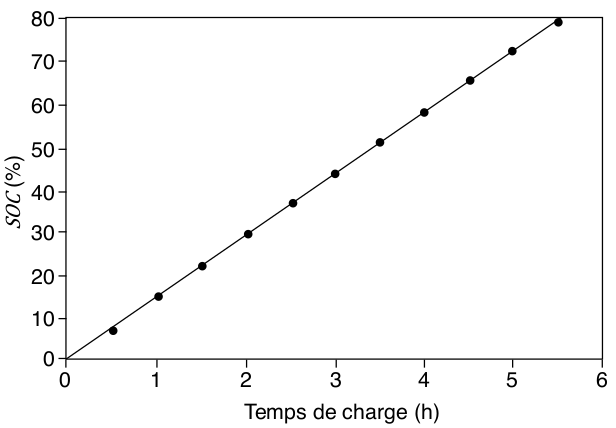
\includegraphics[width=6cm]{Ex22/10-SoC.png}
\end{minipage}\hfill   
\begin{minipage}[c]{0.35\textwidth}     
    \captionof{figure}{\'{E}volution du SoC en fonction du temps de charge.}
    \label{fig:22-03}
\end{minipage}


%\Q Donner le signe de la puissance et du travail lorsqu'une cellule électrochimique est un récepteur reçoit de l'énergie. Même chose si il s'agit d'un générateur.

\paragraph*{Données}
\begin{itemize}
\item \'{E}lectronégativité : $\chi(\ce{Li}) = 0.98$, $\chi(\ce{Co}) = 1.88$ et $\chi(\ce{O}) = 3.44$
\item Masse molaire : $M(C) = 12.0 ~ \si{\gram\per\mole}$
\item Constante de Faraday $F \approx 96.5 \cdot 10^3 \si{\coulomb\per\mole}$
\end{itemize}

